\chapter{Field Patterns for Efficient Objects}
\label{chapter:field-patterns}

[TODO: Fix word wrap in source listings]

In many applications, the heap is filled mostly with instances of just a
few important classes.  You can increase scalability significantly by making these
objects as compact as possible. This chapter describes field usage
patterns that can be easily optimized for space, for example, fields that are
rarely needed, constant fields, and dependent fields. Simple refactoring of
these kinds of fields can sometimes result in big wins.
 

\section{Rarely Used Fields}
\label{sec:rarely-used}

\paragraph{Side Objects}Chapter~\ref{chapter:delegation} presents examples
where delegating fields to another class increases memory cost. However, sometimes delegation can
actually save memory, if you don't have to allocate the delegated object all the
time.

As an example, consider an on-line store with millions of products. 
Most of the products are supplied by the parent company, but
sometimes the store sells products from another company:
\begin{shortlisting} 
class Product {
	String sku;
	String name;
	..
	String alternateSupplierName;
	String alternateSupplierAddress;
	String alternateSupplierSku;
}
\end{shortlisting}
When there is no alternate supplier, the last three fields
are never used. By moving these fields to a separate side class, you can
 save memory, provided the side object is allocated only when
it is actually needed. This is called \emph{lazy allocation}. Here are the 
refactored classes:

\begin{shortlisting} 
class Product {
	String sku;
	String name;
	.. 
	Supplier alternateSupplier;
}

class Supplier {
	String supplierName;
	String supplierAddress;
	String sku;
}
\end{shortlisting}
For products with no alternate supplier, eight bytes are saved per product,
since three fields are replaced by one. Of course, products with an alternate
supplier pay a delegation cost: an extra pointer and object header, totaling 12
bytes. An interesting question is how
much total memory is actually saved? The answer depends on the percentage of products that have an alternate supplier and
need
a side object, which we'll call the \emph{fill rate}. The higher the fill rate, the less memory is 
saved. In fact, if the fill rate is too high, memory is wasted.

Figure~\ref{fig:fill-rate} shows the memory saved for
different fill rates, assuming three fields (12 bytes) are delegated. The most memory that can be
saved is 8 bytes per object on average, when the fill rate is 0\%. That's 67\%
of the size of the fields that were delegated.
When the fill rate is 10\%, only 50\% of the delegated field bytes are saved on
average. When the fill rate is over 40\%, the memory saved is
negative, that is, memory is wasted. The lesson here is that if you aren't sure
what the fill rate is, then using delegation to save memory may end up
backfiring.
\begin{figure}
  \centering
 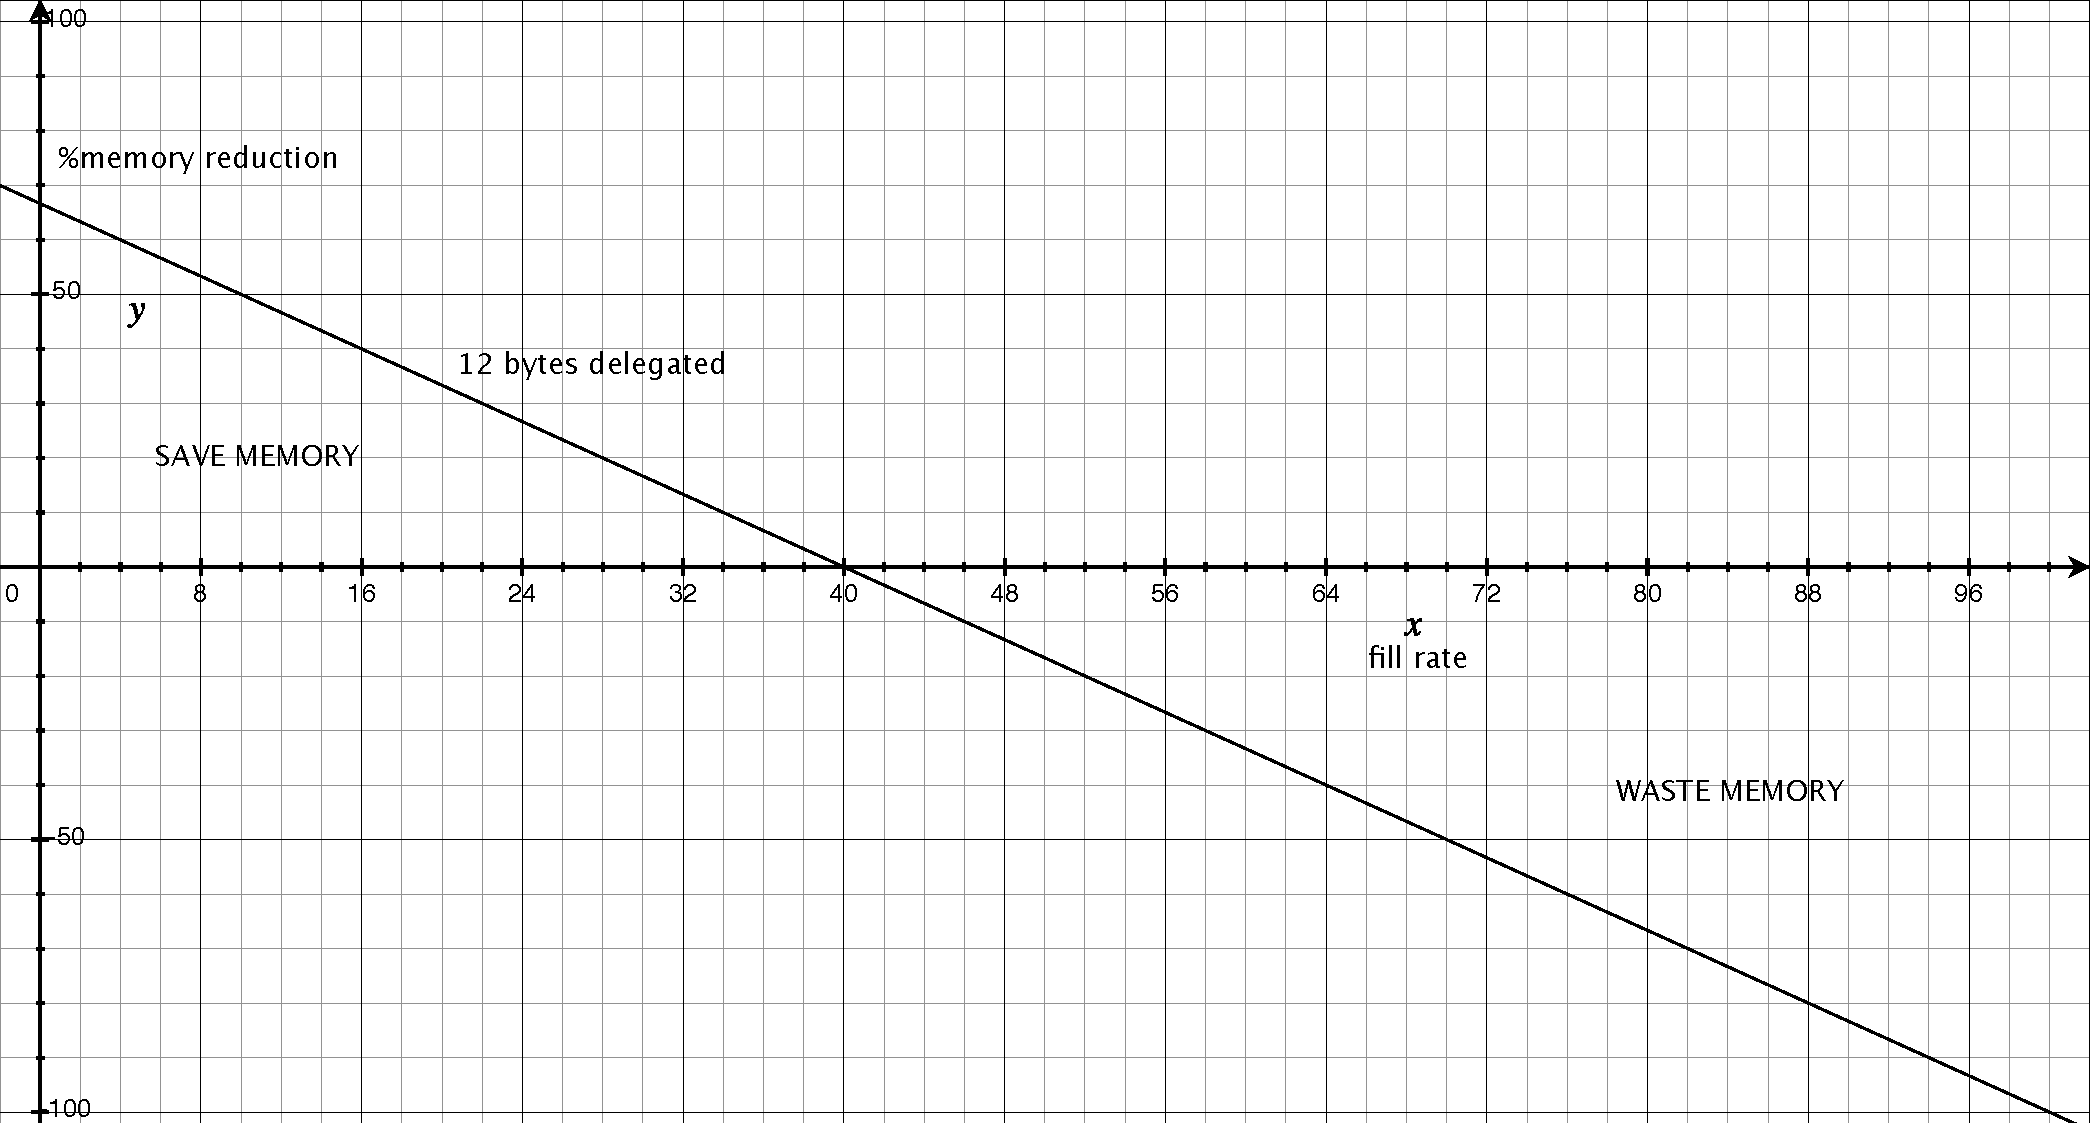
\includegraphics[width=.90\textwidth]{part1/Figures/modelingdatatypes/12-byte-graph.pdf}
 % 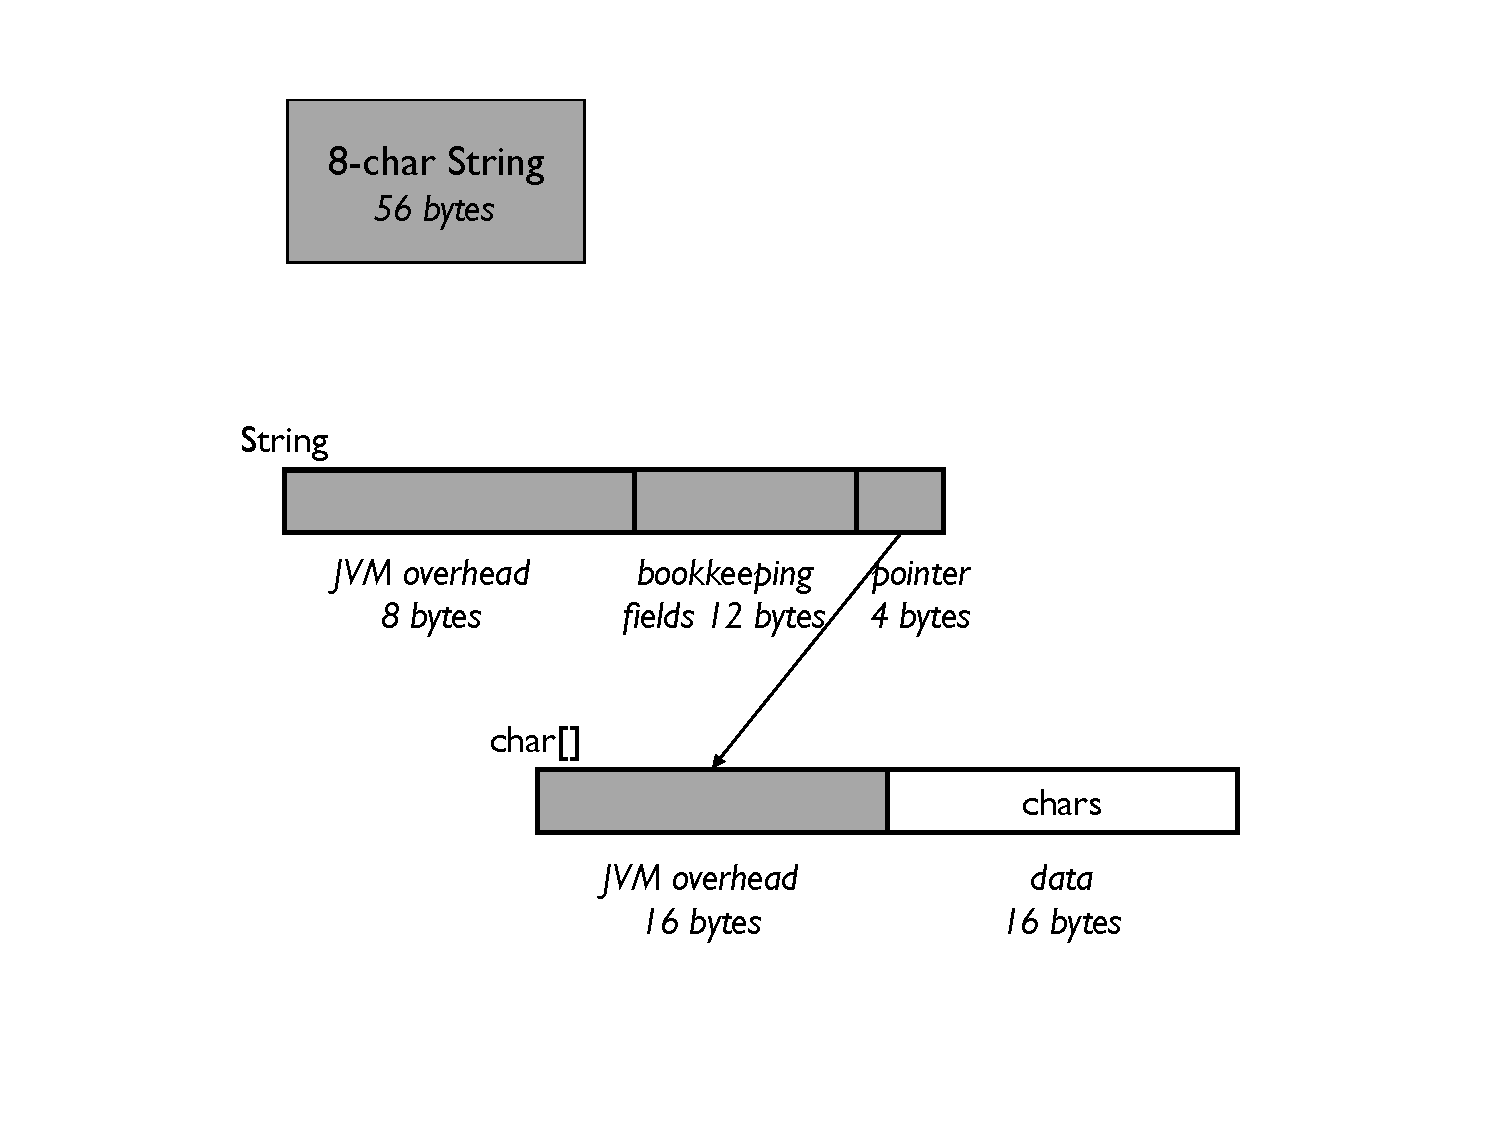
\includegraphics{eight-char-string}
  \caption{This plot shows how much memory is saved or wasted by delegating 12
  bytes of memory to a side object. The x-axis is the fill rate, and the
  y-axis is the average memory saved as a percent of the bytes delegated.}
  \label{fig:fill-rate}
\end{figure}


In addition to the fill rate, the memory savings also depends on the
number of fields delegated and their sizes. The more bytes
delegated, the larger the memory savings, assuming the same fill rate. Figure~\ref{fig:rarely-used} shows the memory
saved or wasted for different fill rates and delegated-field sizes.
Each line represents a different delegated-field size. The bottom-most line
represents a delegated field size of 16 bytes, the next line represents 32 bytes, the next
represents 48 bytes, and so on, up to 144 bytes. As the delegated object size
increases, you can worry less about the fill rate. For example, if 32 bytes
are delegated, there is almost 90\% savings with a low fill rate, and some
memory savings with a fill rate up to 70\%. As the delegation size increases, 
the lines start to converge, since the delegation overhead becomes
less important. At larger sizes there is less of a chance
that underestimating the fill rate will cause you to waste memory, and if it
does, the memory lost will be relatively small.

\begin{figure}
  \centering
 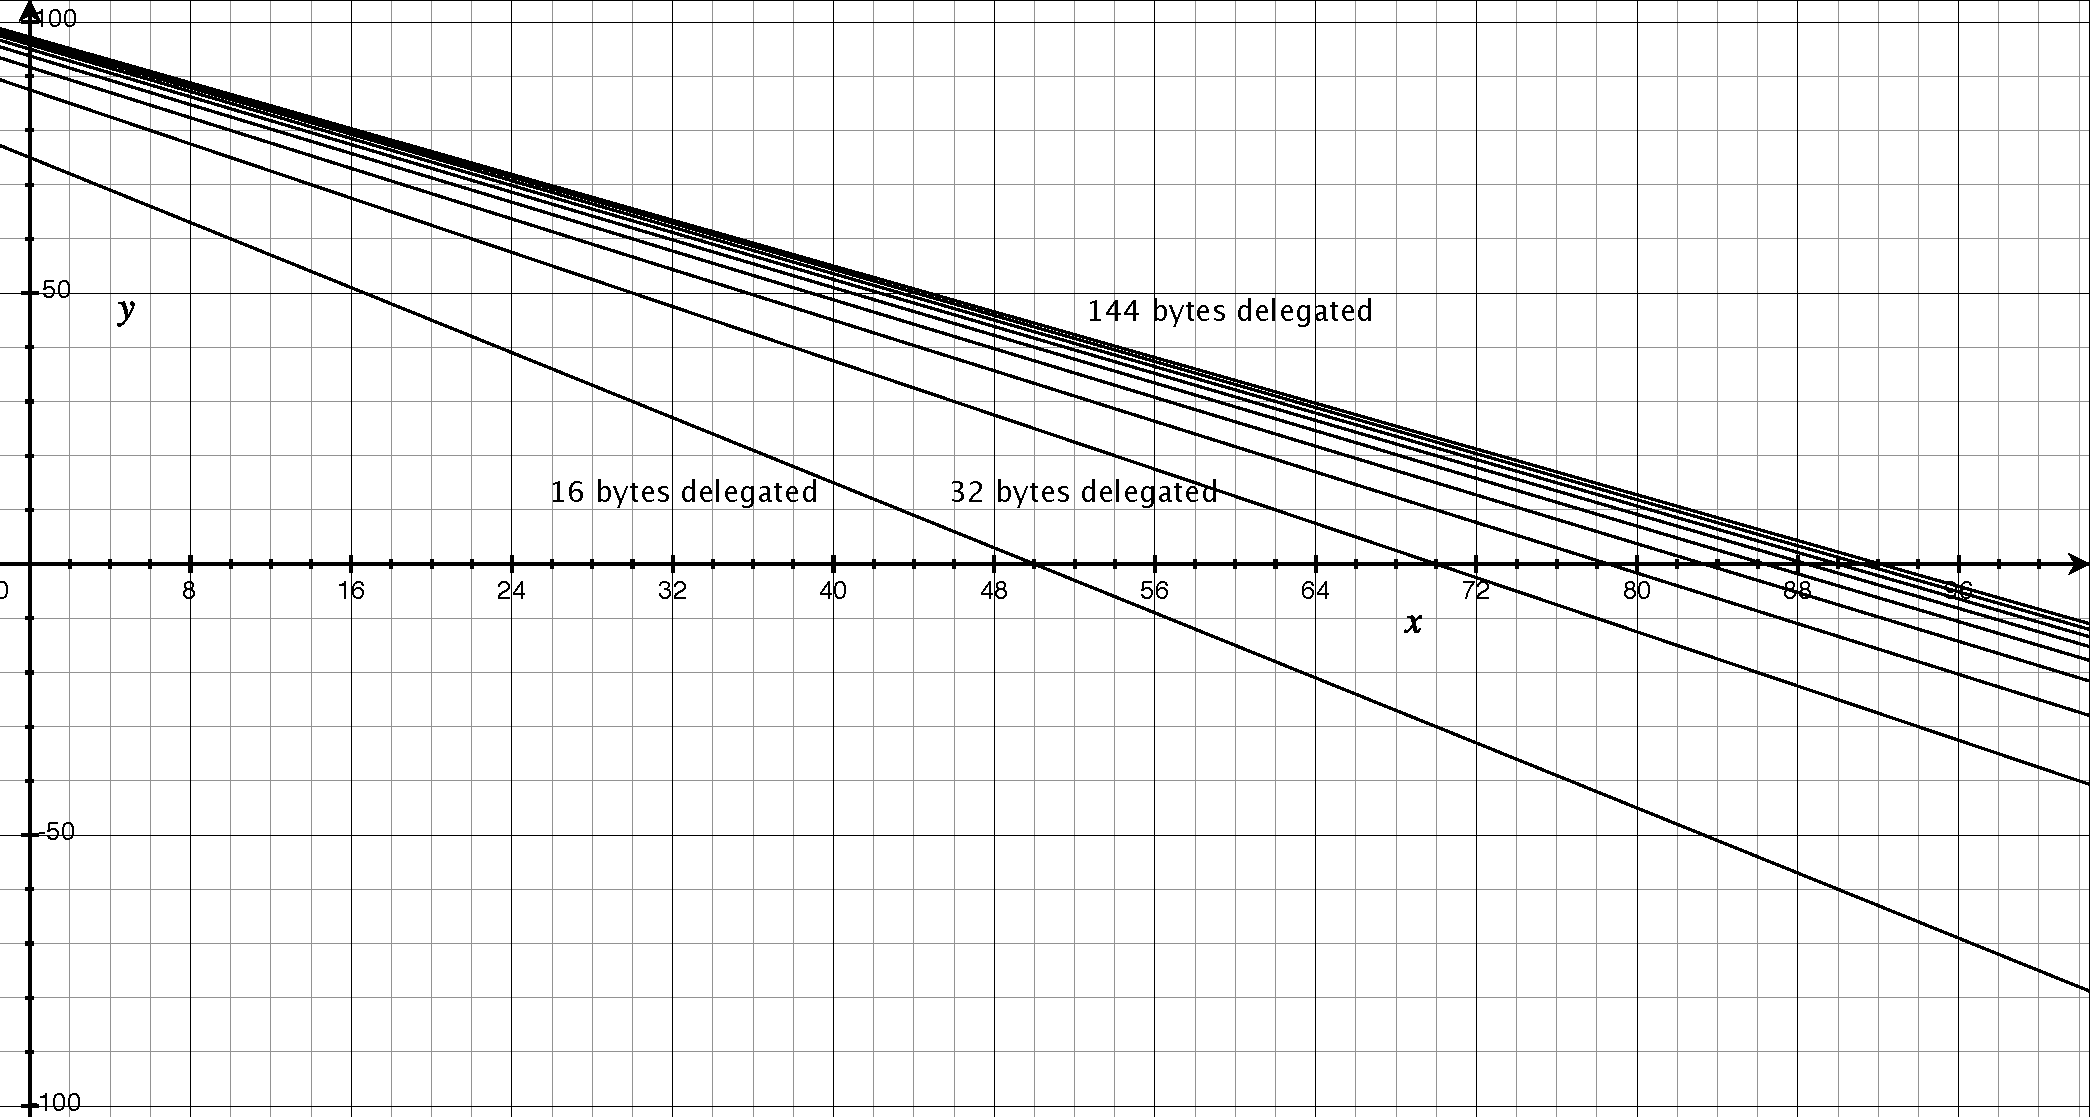
\includegraphics[width=.90\textwidth]{part1/Figures/modelingdatatypes/rarely-used.pdf}
 % 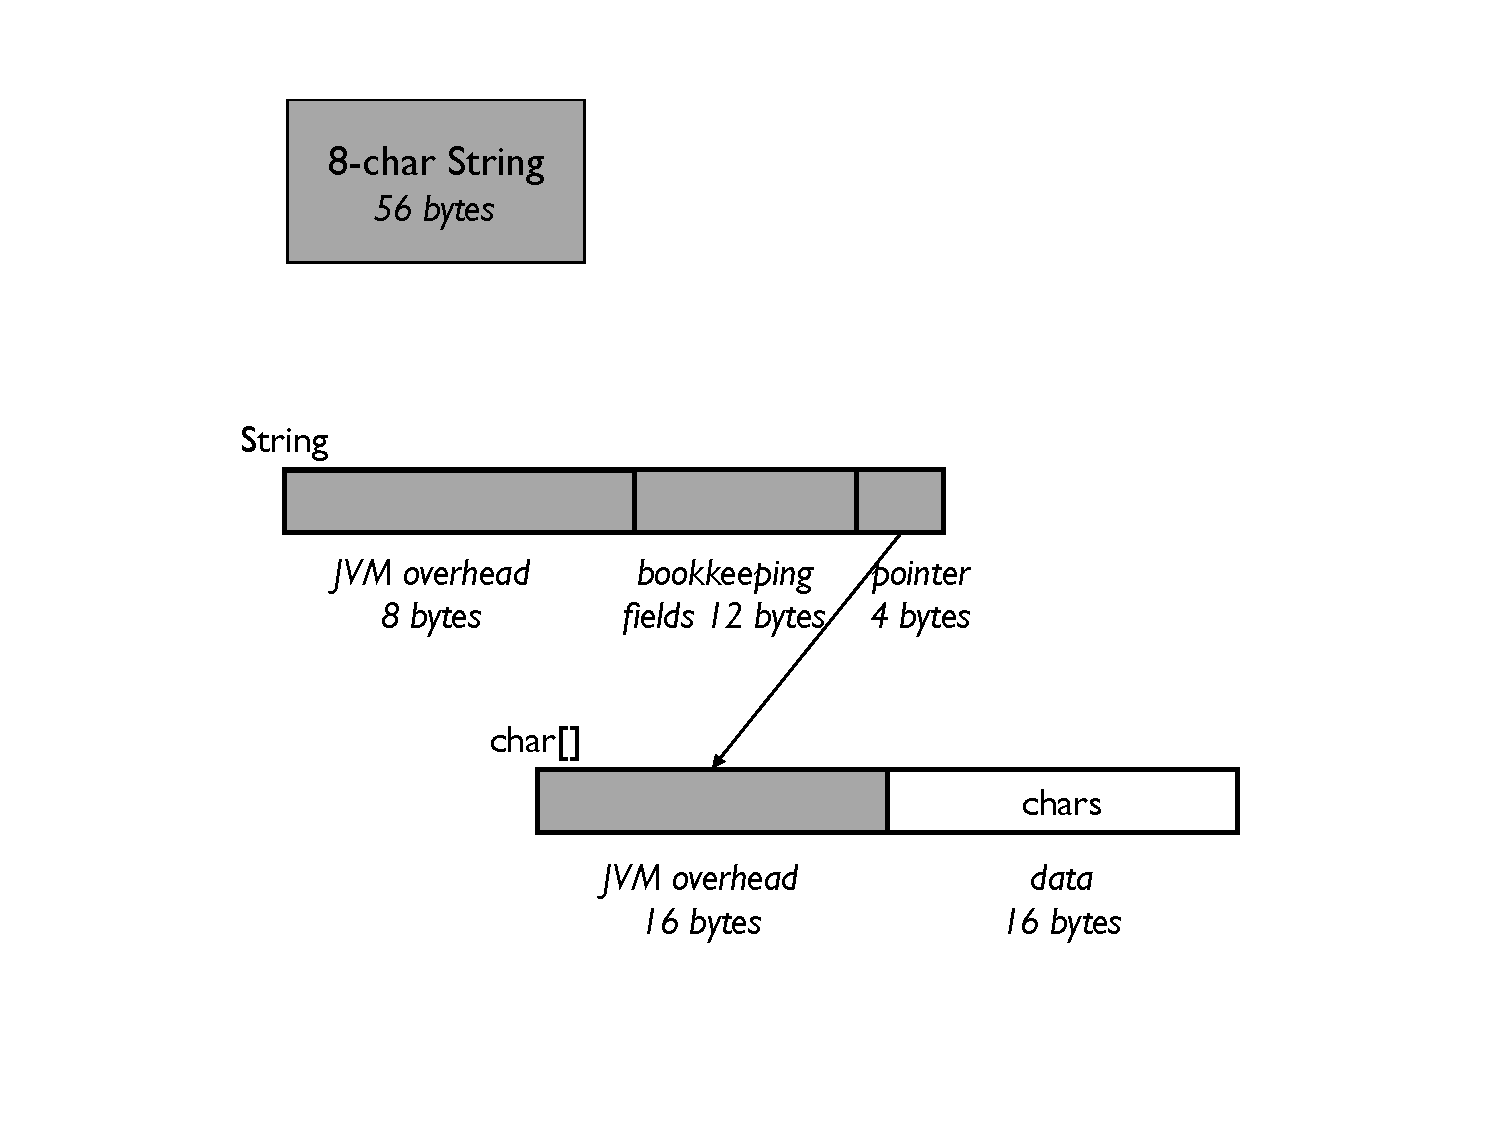
\includegraphics{eight-char-string}
  \caption{This plot shows how much memory is saved or wasted
  depending on how many bytes are delegated to a side object.
  The x-axis is the fill rate, and the y-axis is the average
  memory saved as a percent of the bytes delegated. Each line represents
  a different delegated-fields size, from 16 to 144 bytes, in increments of
  16 bytes.}
  \label{fig:rarely-used}
\end{figure}

\callout{callout:rarely-used}{Delegation Savings Calculation}{
\index{Delegation Savings Calculation}
Assume the cost of a pointer is 4 bytes, and the cost of an object header is 8
bytes.  Let:
\begin{eqnarray} 
B &=& the\ size\ in\ bytes\ of\ the\ delegated\ fields \nonumber \\
F &=& the\ fill\ rate,\ between\ 0\ and\ 1 \nonumber
\end{eqnarray}

While every object pays a
4-byte pointer cost, only F of them pay for a side object. Therefore, using 
a side object will result in an average savings per object of:
\begin{eqnarray}
B-4\ \ -\ \ F(B+8) \nonumber
\end{eqnarray}

For the savings to be positive, the following must be true
\footnote{This calculation does not include alignment overhead.
Delegating fields to a side object may increase alignment costs,
depending on the other fields in your object.
If the header size is not a multiple of the alignment (e.g.
on the IBM 32-bit JRE), delegation can sometimes reduce alignment costs.}:
\begin{eqnarray}
F &<& \frac{B-4}{B+8} \nonumber
\end{eqnarray}

} 
A common error is to put rarely used fields in a side
class with lazy allocation, but have code paths that
cause the side object to be allocated all the time, even when it's not needed.
In this case, instead of saving memory, you pay the full cost of delegation as well as 
the cost of unused fields. 
Lazy allocation
can also be error-prone because it may require testing whether the object
exists at every use. If you need concurrent access to the data in the side
object, you have to take special care to code the checks correctly to avoid race
conditions.
This complexity has to be weighed against potential memory savings.

\paragraph{Side Tables}If a field is very rarely used, then it
might make sense to delete it from its class altogether, and store it in a separate table that maps
objects to attribute values. For example, suppose that only a few of the
products have won major awards, and you want to record this information. Rather than maintaining a field
\code{majorAward} in every product, you can define a table that maps a product
\code{sku} to an award.

\begin{shortlisting}
class Product {
    static HashMap<String, String> majorAward = 
    	new HashMap<String, String>();
    ..
}
\end{shortlisting}

Even though a \class{HashMap} has its own high overhead, this
design can come out ahead if there are a small number of major awards.
You can do a similar analysis as you would for side objects to decide if this
approach is worth it.
A hash entry typically takes more memory than a side object (see
Section~\ref{sec:}).
Therefore, a side table will start wasting
memory at a lower fill rate than would a side object approach.
Whenever you add a new table like this you also have to be careful not to
introduce a memory leak. If products are no longer needed and are garbage
collected, the corresponding entries in the table must be cleaned up.
This topic is discussed at length in Section~\ref{}.

\paragraph{Subclassing} The least expensive way to model rarely used fields
is to move them to a subclass. Unlike the optimizations we've discussed,
subclassing costs no extra space. It can have
some disadvantages from a software engineering standpoint, though, when compared with
delegation or a side table approach. It can make your code less flexible, making
it more difficult to add or rearrange functionality later on. Since Java
supports only single inheritance, defining a subclass for rarely used
fields will prevent you from having subclasses for
other purposes. Using delegation or a side table also allows your data to be more dynamic. 
Rarely used fields can be added after an instance is
created.
 

\section{Mutually Exclusive Fields}
\label{sec:mutually-exclusive}

Sometimes a class has fields that are never used at the same time, and therefore
they can share the same space. Two mutually exclusive fields can be conflated
into one field if they have the same type. Unfortunately, Java does not have
anything like a union type to combine fields of different types. However, if it
makes sense, mutually exclusive field types can be broadened to a common base type
to allow this optimization.

For example, suppose that each women's clothing product has a size, and there
are different kinds of sizes: xsmall-small-medium-large-xlarge,
numeric sizes, petite sizes, and large women's sizes. One way
to implement this is to introduce a field for each kind of size:
\begin{shortlisting}
class WomensClothing extends Product {
	..
	SMLSize      smlSize;
	NumericSize  numSize;
	PetiteSize   petiteSize;
	WomensSize   womensSize; 
}
\end{shortlisting}
Each type is an enum class, such as:
\begin{shortlisting}
enum SMLSize {
	XSMALL, SMALL, MEDIUM, LARGE, XLARGE;
}

enum NumericSize {
	ZERO, TWO, FOUR, SIX, EIGHT, TEN, TWELVE, FOURTEEN, SIXTEEN;
}

enum PetiteSize {
    ZERO, TWO, FOUR, SIX, EIGHT, TEN, TWELVE, FOURTEEN, SIXTEEN;
}

enum WomensSize {
	ONEX, TWOX, THREEX, FOURX;
}
\end{shortlisting}
These four size fields are mutually exclusive --- a clothing item cannot
have both a petite size and a women's size, for example. Therefore, you can
replace these fields by one field, provided that the four enum types are
combined into one enum type:
\begin{shortlisting}
enum ClothingSize {
	XSMALL, SMALL, MEDIUM, LARGE, XLARGE, 
	ZERO, TWO, FOUR, SIX, EIGHT, TEN, TWELVE, FOURTEEN, SIXTEEN,
    PETITE_ZERO, PETITE_TWO, PETITE_FOUR, PETITE_SIX, PETITE_EIGHT, PETITE_TEN,
    PETITE_TWELVE, PETITE_FOURTEEN, PETITE_SIXTEEN,
	ONEX, TWOX, THREEX, FOURX;
}

class Clothing extends Product {
	..
	private ClothingSize     size; 
	..
	public SMLSize getSMLSize() {..}
	public void setSMLSize(SMLSize smlSize) {..}

	public NumericSize getNumericSize() {..}
	public void setNumericSize(NumericSize numericSize) {..}

	public PetiteSize getPetiteSize() {..}
	public void setPetiteSize(PetiteSize PetiteSize) {..}

	public void setNumericSize(WomensSize womensSize) {..}
	public WomensSize getWomensSize() {..}
	..
} 


\end{shortlisting}

You can easily write access and update methods that translate to and from the
original types, so that the caller is insulated from this storage trick.

If the mutually exclusive fields are of different classes,
you can generalize their types by defining a common superclass, if possible.
As a last resort, you can always combine these fields into a single field of type
\class{Object}. Finally, if there are sets of fields that are mutually exclusive, then you can
define a side class for each set of fields, where all side classes have
a common superclass. In this case, you need to do the math to make sure that you
actually save memory, given the extra cost of delegation.

Just like rarely used fields, mutually
exclusive fields can also be modeled using subclassing. Again, the space savings
have to be weighed against other software engineering goals.

\section{Constant Fields}
\label{sec:constant}

Declaring a constant field \code{static} is a simple way to
save memory. Programmers usually remember to make constants like \emph{pi} 
static. There are other situations that are a bit more subtle, for example,
when a field is constant because of how it is used in the context of an
application.

Returning to the product example, suppose that each product has a field
\code{catalog} that points to a store catalog.
If you know that there is always just one store catalog, then the field
\code{catalog} can be turned into a static, saving 4 bytes per product.

As a more elaborate example, suppose that a \class{Product} has a field
referencing a \class{Category} object, where a category may be
books, music, clothes, toys, etc.
Clearly, different products belong to different categories.
However, suppose we define
subclasses \class{Book}, \class{Music}, and \class{Clothing} of the class
\class{Product}, and all instances of a subclass belong to the same category.  
Now the \code{category} field has the same value for products in each subclass,
so it can be declared static:

\begin{shortlisting}
public abstract class Product {
	public abstract Category getCategory();
	..
}

class Book extends Product {
	static Category bookCategory; // Points to the 
                                  // book category object
	public Category getCategory() {return bookCategory;}  
	..
}

class Music extends Product {
	static Category musicCategory; // Points to the
                                   // music category object
	public Category getCategory() {return musicCategory;}  
	..
}

class Clothing extends Product {
	static Category clothingCategory; // Points to the
	                                  // clothing category
                                      // object
	public Category getCategory() {return clothingCategory;}  
	.. 
}

\end{shortlisting}

Knowing the context of how objects are created and used, and how they relate to
other objects, is helpful in making these kinds of memory optimizations.

\section{Nonstatic Member Classes}
Sometimes it is useful to define a class
within a larger class or method. Java lets you create four kinds of
nested classes, each for a different purpose. They are \emph{static member},
\emph{nonstatic member}, \emph{local}, and \emph{anonymous} classes.
Instances of the latter three are always created within the
context of an instance of the enclosing class. Their methods can refer back to
the enclosing instance. To accomplish this, these three kinds of nested classes 
maintain an extra, hidden field, the \code{this} pointer of the enclosing
instance. In contrast, instances of a static member class do not have this extra
field. They are created independently of any instances of the enclosing class.

A common error is to declare a nonstatic member class 
when you don't really need to maintain a link with an
enclosing instance. To illustrate, let's return to the example from Section~\ref{sec:rarely-used},
where we moved some rarely used fields into a side class, \code{Supplier}. 
Suppose we wanted to hide this decision, so that we would have the freedom to change our
minds later if the optimization didn't work out. We could make \code{Supplier} a
member class of Product, as follows:

\begin{shortlisting}
class Product {
	class Supplier {
		String supplierName;
		String supplierAddress;
		String sku;
	}
	
	..
	Supplier alternateSupplier;
	..
	public method void setAlternateSupplierName(String name) {
		// Lazily allocate the alternate supplier object
		if (alternateSupplier == null) {
			alternateSupplier = new Supplier();
		}
		alternateSupplier.supplierName = name;
	}
	..
}
\end{shortlisting}

Since we didn't declare \code{Supplier} to be static, every instance of
\code{Supplier} will contain an extra pointer back to the product which created
it. In cases like this, a static member class can work just as well, and save
the 4-byte pointer field. The only code change is to add the keyword
\code{static} to the declaration of \code{Supplier}.
Notice how Java makes it easy to make this mistake, since the \code{new}
statement that creates an instance of \code{Supplier} looks the same either way.
In the nonstatic case, it hides the fact that it's passing in the enclosing
\code{this} pointer.

The book Effective Java \cite{EffectiveJavaBook} gives the same advice,
to ``favor static member classes over nonstatic'' when you don't need to
maintain a link to the outer instance. It lists more benefits in addition
to the space savings.
For example, the hidden pointer can lead to a memory leak, by
inadvertently holding on to the enclosing instance longer than it's needed. 


\section{Redundant Fields}

A field is redundant if it can be computed on the fly from other fields, and, in
principle, can be eliminated. In the simplest case, two fields store the same
information but in different forms, since the two fields are used for
different purposes. For example, product IDs are
more efficiently compared as \code{ints}, but more easily printed as
\code{Strings}. Since it is possible to convert one representation into the
other, storing both forms is not necessary, and only makes sense if
there is a large performance penalty from performing the data
conversion.
In the more general case, a field may depend on many other values. For example,
you could allocate a field to store the number of items in a shopping cart,
 or simply compute it by adding up all of the shopping cart items. 

There is a trade-off between the performance cost of a conversion or computation
and the memory cost of an extra field, which has to be weighed in context. 
How often is the information needed and how expensive is it to compute? What's
the total memory cost? Comparing performance cost to memory cost is a bit like apples and oranges, 
but often it is clear which resource is most constrained. Here are several
considerations to keep in mind:
\begin{itemize}
  \item Computed \class{String} fields should be used only if there's a good
  reason, since strings have a very high overhead in Java, 
as we have seen.  
\item Computed fields are very useful when storing partial values avoids 
expensive quadratic computations. For example, if you need to support finding
the number of children of nodes in a graph, then caching
this value for each node is a good idea. 
\end{itemize}

If you do need to store a computed field, make sure that you are
using the most efficient representation.  For example,
\class{StringBuffer} is useful for building a character string, but is
less space-efficient than \class{String} for storing the final result.
Chapter~\ref{chapter:representing-values} compares different ways to represent some common
datatypes.
Another thing to watch for is storing many copies of the same computed
value. Even something as simple as storing a large number of empty
\class{String}s can really add up in Java.
Chapter~\ref{chapter:sharing-immutable-data} looks at ways to share
read-only data.

\section{Large Base Classes and Fine-grained Designs}
\index{Base Class Baggage}

As discussed in the previous chapter, highly-delegated data models can result in
too many small objects. Occasionally, you run across a highly-delegated data model where the delegated objects
are large. This can happen when delegated classes inherit from a large base class. When fine grained data modeling
is combined with inheriting from large base classes, memory costs multiply and can become prohibitive.

%\begin{example}{Keeping track of updates} 
A frequent data management requirement is to track creation and update information, that is, when data is created or updated and by whom.  Here is a base class, taken from a real application, that stores create and update information.  
\begin{shortlisting}
class UpdateInfo {
     Date creationDate;
     Party enteredBy;
     Date updateDate;
     Party updatedBy;
}
\end{shortlisting}
You can track changes by subclassing from \class{UpdateInfo}. Update tracking is
a \textit{cross-cutting feature}, since it can apply to any class in a data model.
%\end{example}

Returning to the original, unoptimized
version of \class{EmployeeWithEmergencyContact} in
Section~\ref{fine-grained-data-models}, suppose that updates to employee emergency contacts need to be tracked. 
You need to decide how fine the tracking should be. Should every update to every
phone number and email address be tracked, or is it sufficient to track the fact that some
contact information was changed for an emergency contact? If you decide to
track changes to every contact phone number or email address, you can easily achieve this by
extending the \class{ContactMethod} class defined in the fine-grained data model from Section~\ref{fine-grained-data-models}:
\begin{shortlisting}
class ContactMethod extends UpdateInfo {
     ContactPerson owner;
}
\end{shortlisting}
Figure~\ref{fig:big-base-class} shows an instance of a contact person with
update information associated with every \class{ContactMethod}. Not only is this
a highly delegated structure with multiple \class{ContactMethod} objects, but
each one has an additional 16 bytes. Furthermore, there are potentially four
more objects of type \class{Date} and \class{Party} for each of the four
\class{ContactMethod} objects. A far more scalable solution is to move up a
level, and track changes to each \class{ContactPerson}. With this solution, you
do not need such a fine-grained data model, and the update tracking functionality is 1/4 the cost.
\begin{figure}
  \centering
 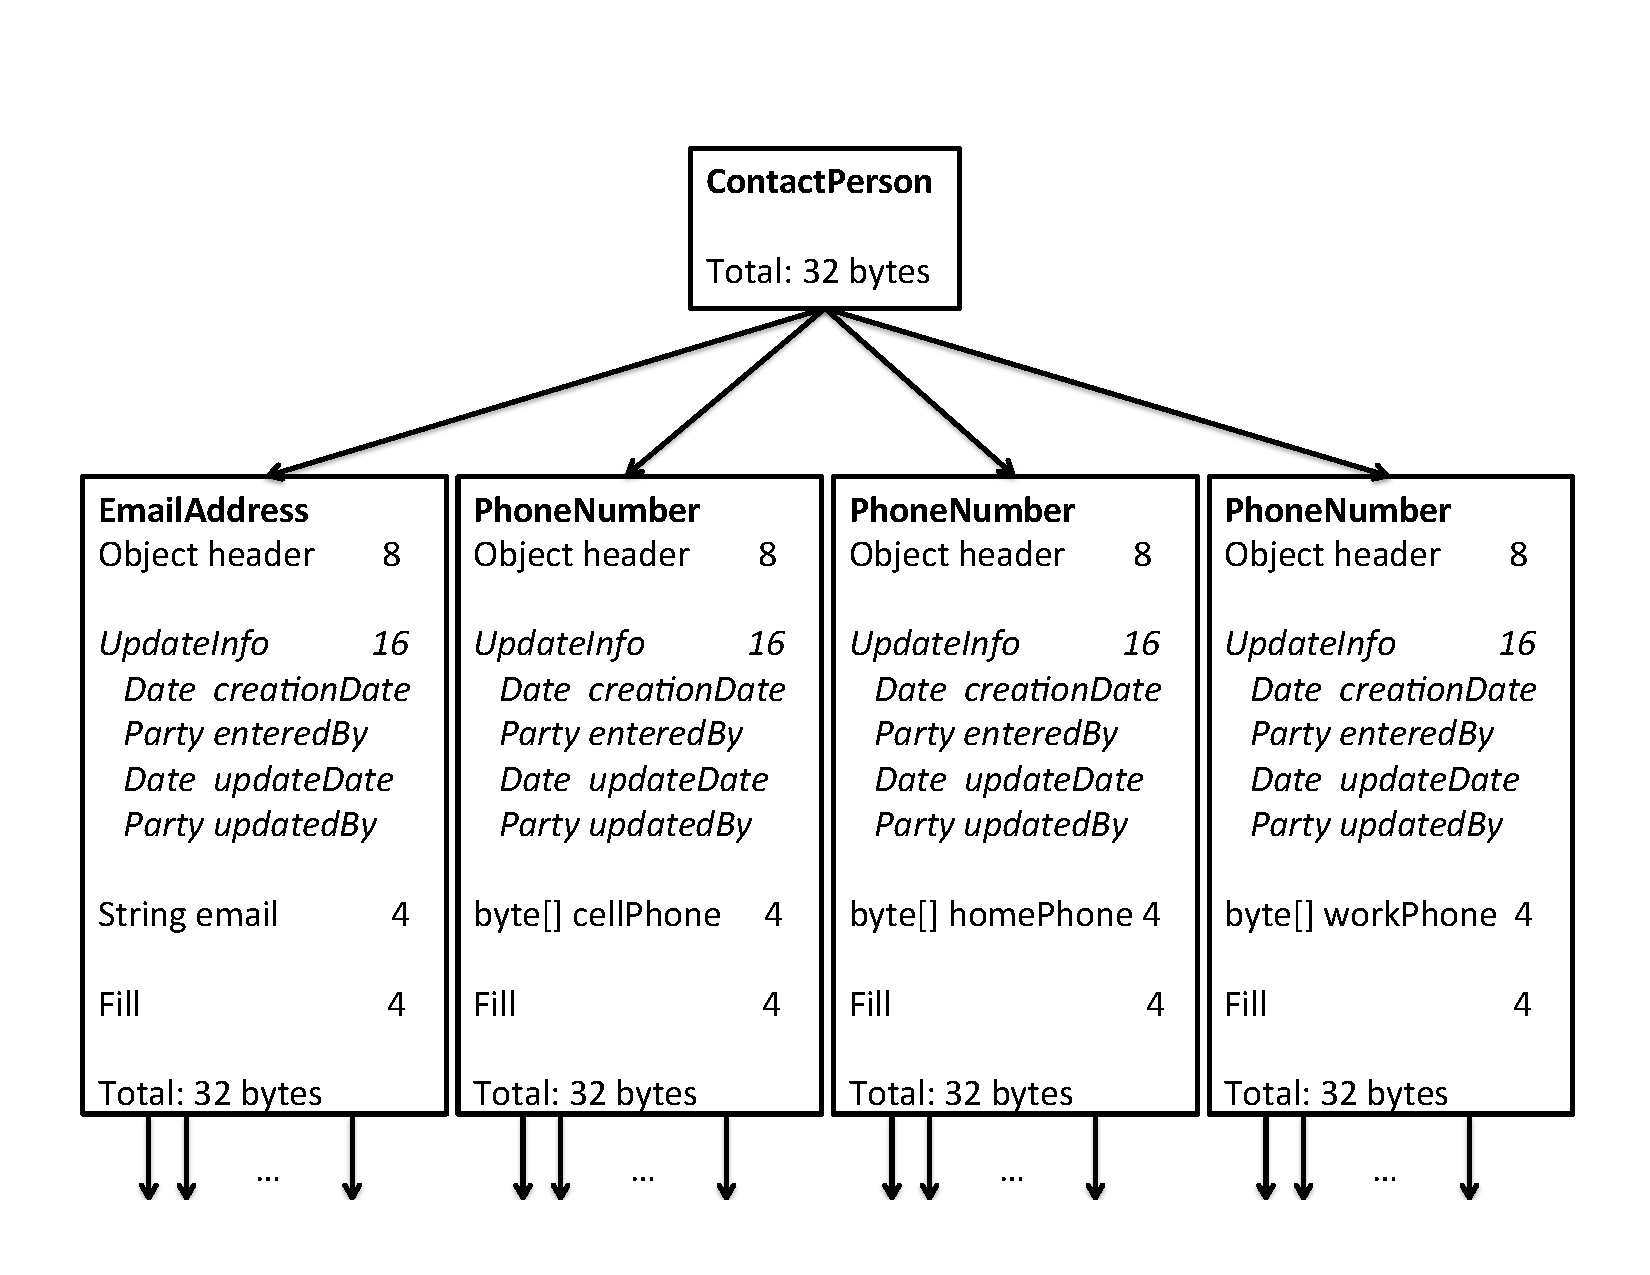
\includegraphics[width=.70\textwidth]{part1/Figures/modelingdatatypes/big-base-class.pdf}
 % 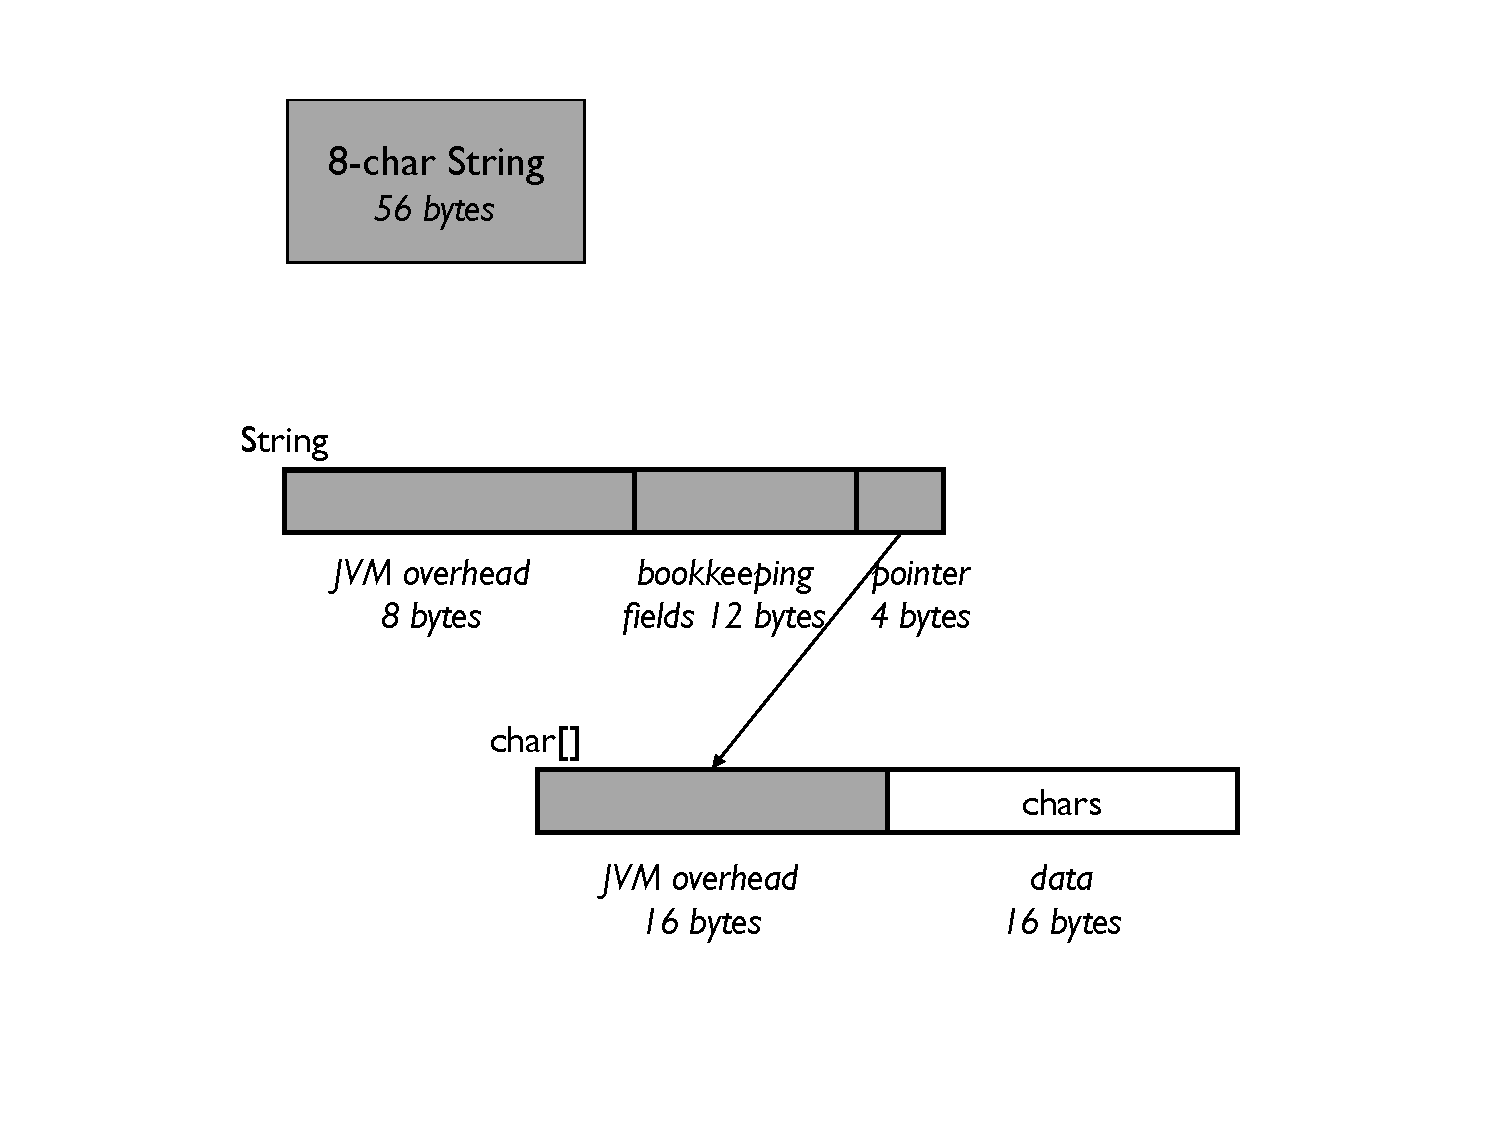
\includegraphics{eight-char-string}
  \caption{The cost of associating \class{UndateInfo} with every
  \class{ContactMethod}.}
  \label{fig:big-base-class}
\end{figure}
 
The solution in Figure~\ref{fig:big-base-class} provides a very fine
granularity of functionality. An argument can be made in favor of this
solution, since you lose functionality and flexibility if you only track
updates to \class{ContactPerson}. However, if the program hits a scalabity
problem, it may not be possible to be this casual with memory. Also, an alternate
design may be available that gives the desired functionality in a more memory-efficient way. In this
example, you could implement an update log instead of tracking updates in the objects themselves. Assuming
updates are sparse, this is a much better solution. It is very easy define a subclass without looking closely
at the memory size of its superclasses, especially if the inheritance chain is
long.



\section{Writing Efficient Framework Code}

The storage optimizations described in this chapter assume that you are
familiar with the entire application you are working on. You need to
understand how objects are created and used, and therefore know enough to determine
whether these optimizations make
sense. However, if you are programming a library or framework, you have no way
of knowing how your code will be used. In fact, your code may be used in a
variety of different contexts with different characteristics. Premature optimization ---
making an assumption about how the code will be used, and optimizing for that
case --- is a common pitfall when programming frameworks.  

For example, suppose the online store is designed as a framework
that can be extended to implement different kinds of stores.
For some stores, most products may have an alternate supplier. For other
stores, most products may not.  There is no way of knowing. If the
\code{Product} class is designed so that the alternate supplier is allocated as
a side object, then sometimes memory will be saved and sometimes wasted. 
One possibility is to define two versions of the \code{Product} class, one that
delegates and one that doesn't. The framework user can then use the version
that is appropriate to the specific context. However, this is generally not
practical. 

Frequently, decisions are made that trade space for time.
There are many instances of this trade-off in the Java standard library. For
example, let�s look at  \code{String}, which has three 
 bookkeeping fields: an offset,
a length, and a hashcode. These 12 bytes of overhead consume 21\% of an eight
character string. 
The offset and length fields implement an optimization for substrings. 
That is, when you create a substring, both
the original string and substring share the same character array, as shown in
Figure~\ref{fig:substring}. The offset and length fields in the substring
\code{String} object specify the shared portion of the character array. 
This scheme optimizes the time to create a substring, since there is no new
character array and no copying. However, every string pays the price of the offset
and length field, whether or not they are used. In practice, most Java applications
have far more strings than substrings\cite{}, so a lot of memory is
wasted. Even when there are many substrings,
if the original strings go away, you have a different footprint problem, namely,
saving character arrays which are too big.
\begin{figure}
  \centering
 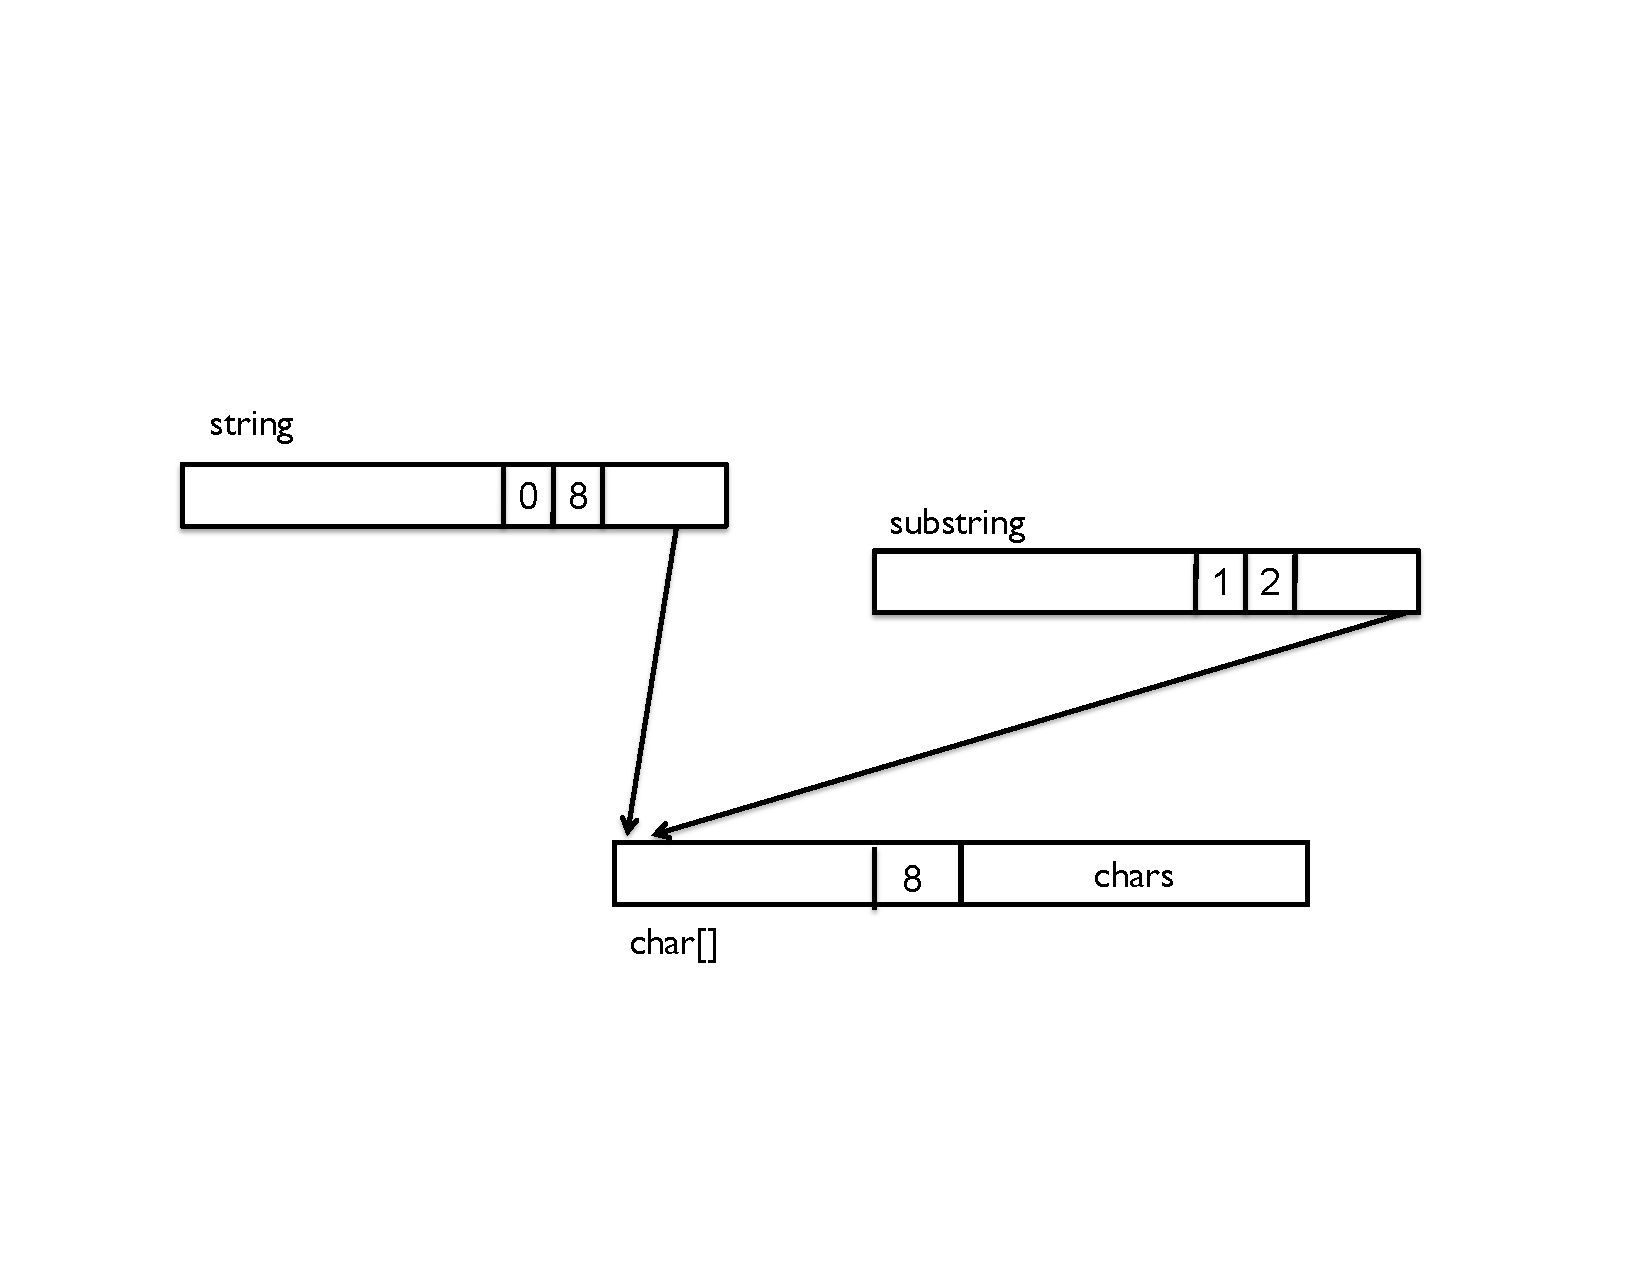
\includegraphics[width=.90\textwidth]{part1/Figures/modelingdatatypes/substring.pdf}
 % 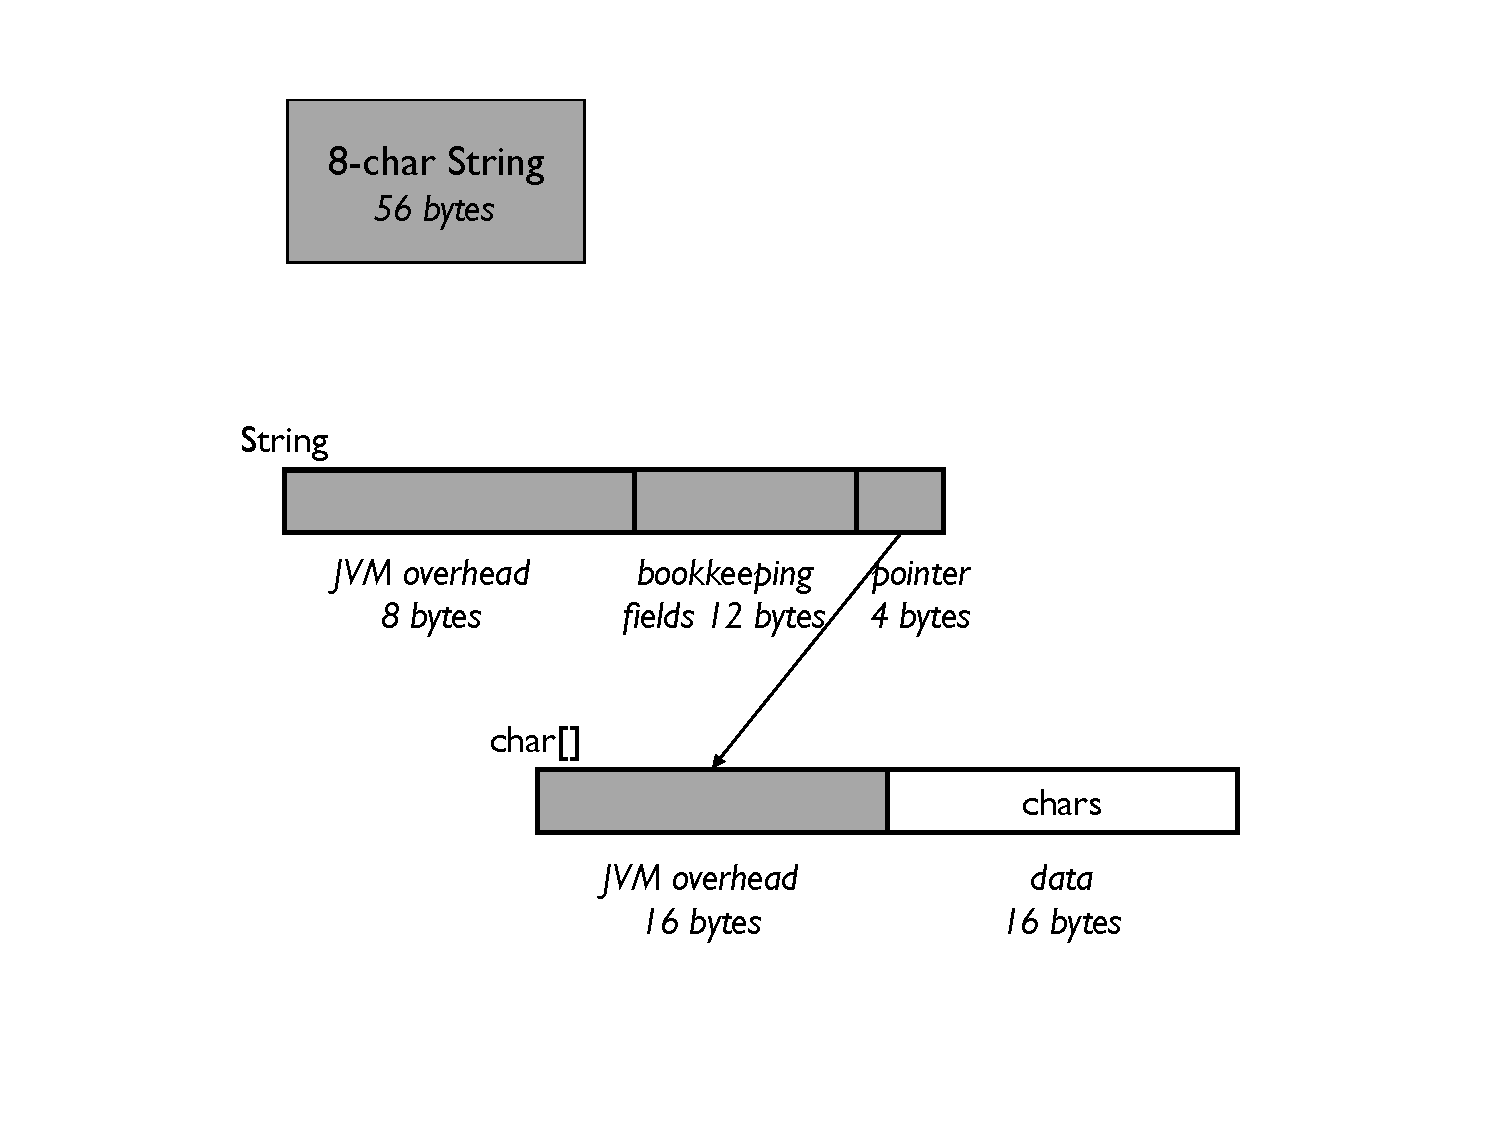
\includegraphics{eight-char-string}
  \caption{A string and a substring share the same character array. The length
  and offset fields are needed only in substrings. In all other strings, the
  offset is 0 and the length is redundant.}
  \label{fig:substring}
\end{figure}

%It says that if I ever take a substring of this thing,
% I�m going to be able to share with the origjnal characters of the String This
 %is a theme you will see throughout the JDK, that there�s so many
% optimizations that are done to avoid copies at any cost. Really with a huge
% focus on time, and almost no focus on space whatsoever. So studies we saw at
% TRL, in reality, in the long liv

The third bookkeeping field in \code{String} is a hashcode.
Storing a hashcode seems like a reasonable idea, since it is expensive to
compute it repeatedly. However, you have to be puzzled by the space-time
trade-off, since 
a string only needs its hashcode when it is stored in a \code{HashSet} or a
\code{HashMap}. In both of these cases, the \code{HashSet} or \code{HashMap}
entry already has a field for hashcode for each element. \footnote{There
may be some benefit in saving the hashcode in a \class{String} that's used for
looking up a map entry, but only when the same \class{String} object is used for
lookup repeatedly.}

This is a cautionary tale of premature optimization. Framework
decisions can have a long-lived impact. At the same time, it is difficult to
test new frameworks in realistic settings, or to even predict how they will be used.
For these \class{String} optimizations, it's not clear that there is any performance gain
in real-world applications, as opposed to benchmarks. Meanwhile all
applications must pay the price in memory footprint.

\section{Summary}

Even though Java does not let you control the layout of objects, it is still
possible to make objects smaller by recognizing certain usage patterns.
Optimization opportunities include:

\begin{itemize}
  \item Rarely used fields can be delegated to a side object, or stored in a
  completely separate attribute table.
  \item Mutually exclusive fields can share the same field, provided they have
  the same type.
  \item Fields that have the same value in all instances of a class can be
  declared static.
  \item Redundant fields whose value depends on the value of other fields can
  be eliminated, and recomputed each time they are used.
  \item Inner classes which can be made static will avoid storing a
  hidden \code{this} pointer. 
\end{itemize}

Every field eliminated saves around 4 bytes per object, which may seem small.
However, often several optimizations can be applied to a class, and if the
class has a lot of instances, then these small
optimizations turn out to be significant. They are especially useful in
base classes, where their effect can be multiplied.

Many of these optimizations do not come for free. They trade one kind of cost
for another, and can easily make things worse, depending on the context.
So it's important to look at how your data will be used, and to estimate
and then measure the effect of any optimizations. It's also a good idea to
design your APIs so that classes can be easily refactored
later on:

\begin{itemize}
  \item Callers use interfaces rather than concrete classes.
  \item Callers use factory methods rather than constructors.
\end{itemize}

